\subsection{UC 10 - Amministrazione - Gestione enti}

		\begin{figure}[H]
			\centering
			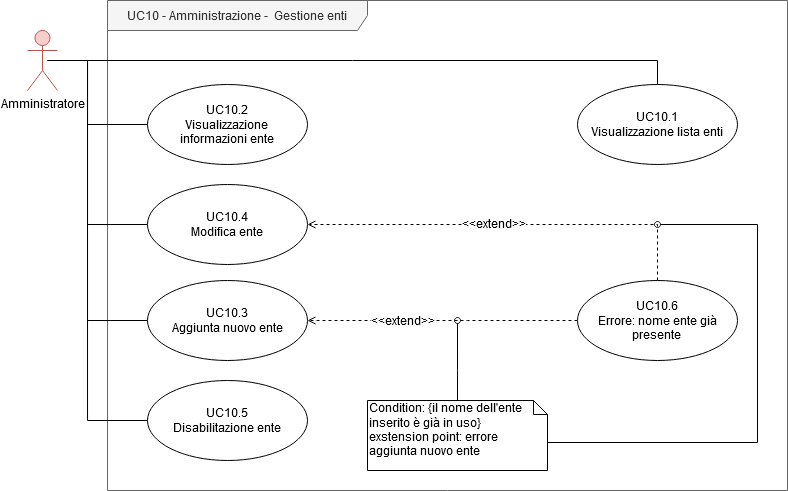
\includegraphics[scale=0.60]{res/images/uc10}
			\caption{Diagramma che descrive la gestione degli enti a livello amministrativo.}
		\end{figure}

		\begin{itemize}
			\item \textbf{Attori Primari}: Amministratore.
			\item \textbf{Descrizione}: L'utente può gestire gli enti del sistema, visualizzando la lista completa, aggiungendone di nuovi, modificandone di esistenti e rimuovendone all'occorrenza.
			\item \textbf{Precondizione}: L'utente naviga nella gestione enti per l'amministrazione.
			\item \textbf{Postcondizione}: L'utente ha visualizzato o gestito gli enti all'interno del sistema. 
			\item \textbf{Scenario Principale}:
			\begin{enumerate}
				\item{L'utente visualizza o gestisce gli enti all'interno del sistema.}
			\end{enumerate}	
		\end{itemize}

			\subsubsection{UC 10.1 - Visualizzazione lista enti }
			\begin{itemize}
				\item \textbf{Attori Primari}: Amministratore.
				\item \textbf{Descrizione}: L'utente può visualizzare la lista degli enti attivi censiti nel sistema.
				\item \textbf{Precondizione}: L'utente naviga nella gestione enti per l'amministrazione.
				\item \textbf{Postcondizione}: L'utente ha visualizzato la lista degli enti presenti nel sistema.
				\item \textbf{Scenario Principale}:
				\begin{enumerate}
					\item{L'utente visualizza la lista enti attualmente attivi e disponibili.}
				\end{enumerate}	
			\end{itemize}

			\subsubsection{UC 10.2 - Visualizzazione informazioni ente}
			\begin{itemize}
				\item \textbf{Attori Primari}: Amministratore.
				\item \textbf{Descrizione}: L'utente può visualizzare le informazioni riguardanti uno specifico ente, quali il suo nome, il nome per esteso e il luogo della sede.
				\item \textbf{Precondizione}: L'utente naviga nella gestione enti per l'amministrazione.
				\item \textbf{Postcondizione}: L'utente visualizza le informazioni di un ente selezionato.
				\item \textbf{Scenario Principale}:
				\begin{enumerate}
					\item{L'utente seleziona dalla lista un ente}
					\item{L'utente visualizza le informazioni riguardanti l'utente selezionato}
				\end{enumerate}	
			\end{itemize}

			\subsubsection{UC 10.3 - Aggiunta nuovo ente}
			\begin{itemize}
				\item \textbf{Attori Primari}: Amministratore.
				\item \textbf{Descrizione}: L'utente può aggiungere un nuovo ente al sistema, inserendo le apposite informazioni richieste.
				\item \textbf{Precondizione}: L'utente naviga nella gestione enti per l'amministrazione.
				\item \textbf{Postcondizione}: L'utente ha creato un nuovo ente.
				\item \textbf{Scenario Principale}:
				\begin{enumerate}
					\item{L'utente deve compilare dei campi per proseguire con l'inserimento di un nuovo ente;}
					\item L'utente inserisce il nome ente (UC 10.3.1);
					\item L'utente inserisce la sede (luogo) in cui risiede l'ente (UC 10.3.2);
					\item{L'ente viene creato dall'utente con le informazioni fornite.}
				\end{enumerate}	
				\item \textbf{Estensioni}:
					\begin{itemize}
						\item Errore: il nome ente inserito è già presente (UC 10.6)
					\end{itemize}
			\end{itemize}	

				\paragraph{UC 10.3.1 - Inserimento nome ente}
				\begin{itemize}
					\item \textbf{Attori Primari}: Amministratore.
					\item \textbf{Descrizione}: L'utente sta aggiungendo un nuovo ente al sistema e deve compilare il campo per il nome dell'ente.
					\item \textbf{Precondizione}: L'utente sta aggiungendo un nuovo ente e deve compilare un campo specifico.
					\item \textbf{Postcondizione}: L'utente ha compilato il campo specifico.
					\item \textbf{Scenario Principale}:
					\begin{enumerate}
						\item L'utente inserisce il nome ente.
					\end{enumerate}	
				\end{itemize}	

				\paragraph{UC 10.3.2 - Inserimento della sede}
				\begin{itemize}
					\item \textbf{Attori Primari}: Amministratore.
					\item \textbf{Descrizione}: L'utente sta aggiungendo un nuovo ente al sistema e deve compilare il campo per la sede dell'ente.
					\item \textbf{Precondizione}: L'utente sta aggiungendo un nuovo ente e deve compilare un campo specifico.
					\item \textbf{Postcondizione}: L'utente ha compilato il campo specifico.
					\item \textbf{Scenario Principale}:
					\begin{enumerate}
						\item L'utente inserisce la sede in cui risiede l'ente.
					\end{enumerate}	
				\end{itemize}			

			\subsubsection{UC 10.4 - Modifica ente}
			\begin{itemize}
				\item \textbf{Attori Primari}: Amministratore.
				\item \textbf{Descrizione}: L'utente può modificare un ente esistente nel sistema, inserendo le apposite informazioni richieste.
				\item \textbf{Precondizione}: L'utente naviga nella gestione enti per l'amministrazione.
				\item \textbf{Postcondizione}: L'utente ha modificato l'ente che aveva selezionato.
				\item \textbf{Scenario Principale}:
				\begin{enumerate}
					\item L'utente seleziona un ente specifico da quelli disponibili;
					\item{L'utente deve compilare dei campi per proseguire con la modifica di un ente esistente;}
					\item L'utente modifica il nome ente (UC 10.4.1);
					\item L'utente modifica la sede (luogo) in cui risiede l'ente (UC 10.4.2);
					\item{L'ente viene creato dall'utente con le informazioni fornite.}
				\end{enumerate}	
				\item \textbf{Estensioni}:
					\begin{itemize}
						\item Errore: il nome ente inserito è già presente (UC 10.6)
					\end{itemize}
			\end{itemize}	

				\paragraph{UC 10.4.1 - Modifica nome ente}
				\begin{itemize}
					\item \textbf{Attori Primari}: Amministratore.
					\item \textbf{Descrizione}: L'utente sta modificando un ente presente nel sistema e deve compilare il campo per il nome dell'ente.
					\item \textbf{Precondizione}: L'utente sta modificando un ente e deve compilare un campo specifico.
					\item \textbf{Postcondizione}: L'utente ha compilato il campo specifico.
					\item \textbf{Scenario Principale}:
					\begin{enumerate}
						\item L'utente modifica il nome ente.
					\end{enumerate}	
				\end{itemize}	

				\paragraph{UC 10.4.2 - Modifica della sede}
				\begin{itemize}
					\item \textbf{Attori Primari}: Amministratore.
					\item \textbf{Descrizione}: L'utente sta modificando un ente presente nel sistema e deve compilare il campo per la sede dell'ente.
					\item \textbf{Precondizione}: L'utente sta modificando un ente e deve compilare un campo specifico.
					\item \textbf{Postcondizione}: L'utente ha compilato il campo specifico.
					\item \textbf{Scenario Principale}:
					\begin{enumerate}
						\item L'utente modifica la sede in cui risiede l'ente.
					\end{enumerate}	
				\end{itemize}	


			\subsubsection{UC 10.5 - Disabilitazione ente}
			\begin{itemize}
				\item \textbf{Attori Primari}: Amministratore.
				\item \textbf{Descrizione}: L'utente può disabilitare un ente dal sistema dal sistema.
				\item \textbf{Precondizione}: L'utente visualizza la lista degli enti appartenenti al sistema.
				\item \textbf{Postcondizione}: L'utente ha disabilitato l'ente selezionato.
				\item \textbf{Scenario Principale}:
				\begin{enumerate}
					\item{L'utente seleziona l'ente da disabilitare;}
					\item{L'utente non visualizza più l'ente selezionato.}
				\end{enumerate}	
			\end{itemize}	

			\subsubsection{UC 10.6 - Errore: nome ente già presente}
			\begin{itemize}
				\item \textbf{Attori Primari}: Amministratore.
				\item \textbf{Descrizione}: L'utente, dopo aver compilando il campo per il nome di un ente, visualizza un errore che segnala che il nome ente è già censito nel sistema.
				\item \textbf{Precondizione}: L'utente ha compilato il nome dell'ente.
				\item \textbf{Postcondizione}: L'utente visualizza un errore specifico e non porta a termine l'azione intrapresa.
				\item \textbf{Scenario Principale}:
				\begin{enumerate}
					\item{L'utente conferma i campi compilati, tra cui quello per il nome ente;}
					\item{Viene visualizzato un errore che segnala la presenza all'interno del sistema di un ente con lo stesso nome.}
				\end{enumerate}	
			\end{itemize}			